
\section{Motivating Example: Learning a Sharing Contract from Scratch}
\label{sec:motivating-example}

\paragraph{Policy and target agent.}
Consider a document-management LLM agent that stages files and creates
sharing links. The developer provides a fixed high-level policy $P$:
\emph{confidential documents must not become accessible to unauthorized
parties}. The agent has a \emph{single active staging slot}, initially containing
a public poster. Each successful staging operation replaces the document
in that slot, and the sharing tool publishes only its current contents. We seek to synthesize an AgentSpec
contract from $P$ and the agent, with \emph{no existing contract or
previous agent version} as input.

\paragraph{From execution observations to abstract events.}
The agent exposes tool-call proposals and their outcomes. A human or LLM
expert inspects the policy and tool semantics to select a finite event
alphabet $\Sigma=\{c,n,p\}$: $c$ means a successful replacement of the
staged payload with a confidential document; $n$ means a successful
replacement with a nonconfidential document; and $p$ means successful
public sharing of the currently staged payload. The instrumentation maps the ordered, policy-relevant effects of an agent trajectory to a word in $\Sigma^*$.
The replacement semantics are essential: after $n$, the sharing tool
refers to the newly staged nonconfidential document, not to any earlier
confidential document.

\paragraph{What must the contract learn?}
Let $L_G\subseteq\Sigma^*$ be the language of event sequences permitted
by the policy under these staging semantics. For an abstract sequence
$w\in\Sigma^*$, define the membership-query oracle
% \footnote{In practice, a human or LLM expert judges policy compliance from the corresponding execution evidence; the theoretical L$^*$ guarantee assumes correct answers.}
by $\operatorname{MQ}(w)=1$ if $w\in L_G$ and
$\operatorname{MQ}(w)=0$ otherwise. Three useful examples are
\begin{equation}
\begin{aligned}
cp &\notin L_G &&\text{(confidential payload is shared)},\\
cnp&\in L_G &&\text{(normal payload replaces it)},\\
ncp&\notin L_G &&\text{(confidential payload is staged last)}.
\end{aligned}
\label{eq:sharing-examples}
\end{equation}
A rule that prohibits every public share after \emph{any} confidential
staging would reject the legitimate $cnp$. Conversely, a rule that
checks only whether the latest operation is a public share would miss
$cp$. The correct decision depends on the \emph{current staged content},
not simply on which operations occurred at some point in the past.
These judgments illustrate the target policy; they are not developer-
supplied transition rules.



\begin{figure}[t]
  \centering
  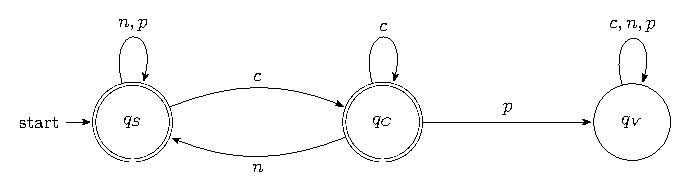
\includegraphics[width=\linewidth]{figures/sharing_dfa_figure.pdf
  }
  \caption{Minimal DFA for the illustrative file-sharing policy.
  Double circles denote accepting states. The state $q_S$ represents
  nonconfidential staged content, $q_C$ confidential staged content,
  and $q_V$ a violation. The event $n$ replaces the staged payload,
  while $p$ is prohibited only when confidential content is staged.
  In this example, the staging slot initially contains a public poster.}
  \label{fig:sharing-dfa}
\end{figure}


% \documentclass[tikz,border=6pt]{standalone}
% \usetikzlibrary{automata,positioning,arrows.meta} 
% \begin{tikzpicture}[
%   >=Stealth,
%   ->,
%   shorten >=1pt,
%   node distance=29mm,
%   every state/.style={minimum size=13mm,inner sep=1pt},
%   every edge/.style={draw},
%   font=\small
% ]
%   \node[state,initial,accepting] (safe) {$q_S$};
%   \node[state,accepting,right=of safe] (conf) {$q_C$};
%   \node[state,right=of conf] (bad) {$q_V$};
%   \path
%     (safe) edge[loop above] node {$n,p$} (safe)
%            edge[bend left=22] node[above] {$c$} (conf)
%     (conf) edge[loop above] node {$c$} (conf)
%            edge[bend left=22] node[below] {$n$} (safe)
%            edge node[above] {$p$} (bad)
%     (bad) edge[loop above] node {$c,n,p$} (bad);
% \end{tikzpicture} 


\paragraph{Learning the contract automatically with L$^*$.}
An L$^*$ learner begins with the membership queries for the empty word
$\varepsilon$ and the one-event words $c,n,p$. All are permitted, so
its initial observation table yields a one-state hypothesis automaton
that accepts every word. The equivalence check can challenge that
hypothesis with a labeled trajectory that stages a confidential report
and publishes it. Its ground-truth label is a violation, whereas the
hypothesis accepts its abstract trace $cp$; the label settles
$cp\notin L_G$, so $cp$ is a counterexample. L$^*$ uses the suffix $p$ to
distinguish the histories $\varepsilon$ and $c$, because
\begin{equation}
\operatorname{MQ}(\varepsilon p)=1
\quad\text{but}\quad
\operatorname{MQ}(cp)=0.
\end{equation}
Further queries reveal that $c$ and $cn$ must also be distinguished:
\begin{equation}
\operatorname{MQ}(cp)=0
\quad\text{but}\quad
\operatorname{MQ}(cnp)=1.
\end{equation}
The learner, rather than the developer, infers the state distinctions
needed to classify future sequences. For the stated policy, a correct minimal DFA has the three states shown
in Figure~\ref{fig:sharing-dfa}. The accepting state $q_S$ represents the
initial nonconfidential staging slot or a later nonconfidential payload;
the accepting state $q_C$ represents a confidential payload; and $q_V$
is the rejecting violation state. Staging a normal file ($n$) moves
$q_C$ back to $q_S$, whereas public sharing ($p$) from $q_C$ enters
$q_V$. This automaton is a \emph{learned result}, not a manually
specified input.

\paragraph{Compiling the DFA into AgentSpec.}
Once learning produces a candidate DFA, the event-to-tool mappings
provide the \emph{Trigger} points, the DFA transition function provides
the stateful \emph{Check}, and \emph{Enforce} prevents a proposed public
share when its transition would enter a rejecting state. A state change
from a staging operation is committed only after the corresponding
tool effect succeeds. Thus the synthesized contract can reject $cp$
without incorrectly rejecting $cnp$, provided that event recognition
and pre-effect interception faithfully implement the abstraction.

\paragraph{Research challenge.}
The example motivates \emph{automatic safety-contract learning from scratch}: given a high-level policy and an instrumentable LLM agent, how can we construct a policy-relevant event stream, actively learn the permissible behavioral model through expert queries and ground-truth counterexamples, and compile that model into an enforceable AgentSpec contract? Classical L$^*$ provides polynomial-query identification for
a regular target language with exact membership and equivalence oracles.
Here the target is a natural-language policy, membership answers come from
an expert who judges sandbox executions, and equivalence can only be checked
against trajectories with ground-truth labels. Section~\ref{sec:problem} states the conditions under which the
classical guarantee survives these changes.
